% Jig vision report, the short picture version: which method, the procedure step by step in the simulator, program v10.
% Build: python walkthrough_figs.py && latexmk -pdf jig_vision_report.tex
% The long text version with every number: jig_vision_report_detailed.tex
\documentclass[11pt,a4paper]{article}

\usepackage[utf8]{inputenc}
\usepackage[T1]{fontenc}
\usepackage[margin=16mm,top=20mm]{geometry}
\usepackage{graphicx}
\usepackage{booktabs}
\usepackage[table,dvipsnames]{xcolor}
\usepackage[font=small,labelfont=bf]{caption}
\usepackage{hyperref}
\usepackage{fancyhdr}
\usepackage{enumitem}
\usepackage{tcolorbox}

\definecolor{hdrblue}{HTML}{2F6FB5}
\definecolor{rowlt}{HTML}{EFF3F8}
\hypersetup{colorlinks=true,linkcolor=hdrblue,urlcolor=hdrblue}
\pagestyle{fancy}
\fancyhf{}
\fancyhead[L]{\small MMA4002 DAM -- Robot cell: finding the jigs with a camera}
\fancyhead[R]{\small\thepage}
\renewcommand{\headrulewidth}{0.4pt}
\setlist{itemsep=0pt,topsep=2pt}
\setlength{\parindent}{0pt}
\newcommand{\hdr}[1]{\textcolor{white}{\textbf{#1}}}
\newcommand{\code}[1]{\texttt{\small #1}}
\newcommand{\step}[1]{\par\medskip{\large\textbf{\color{hdrblue}#1}}\par\smallskip}

% generated by walkthrough_figs.py from walkthrough_20261117-104533
\newcommand{\wtRun}{walkthrough\_20261117-104533}
\newcommand{\wtPhotos}{15}
\newcommand{\wtRms}{0.048}
\newcommand{\wtHePos}{0.20}
\newcommand{\wtHeFound}{0.0, 75.0, 52.8}
\newcommand{\wtMeasMax}{0.26}
\newcommand{\wtTipMax}{0.94}
\newcommand{\wtTipMed}{0.37}
\newcommand{\wtVnineMax}{91}
\newcommand{\wtMoves}{117}
\newcommand{\wtCollNine}{fixtures free, parts 5 moves collide}
\newcommand{\wtCollTen}{fixtures free, parts free}
\newcommand{\wtAsmEvents}{22}
\newcommand{\wtAsmState}{finished}
\newcommand{\wtSetA}{-44/+42\,mm +11\,°}
\newcommand{\wtGotA}{-43.3/+28.7\,mm +11.2\,°}
\newcommand{\wtSetB}{-29/-1\,mm -2\,°}
\newcommand{\wtGotB}{-28.9/+1.4\,mm -2.1\,°}
\newcommand{\wtSetR}{+0/+0\,mm +0\,°}
\newcommand{\wtGotR}{no marker (stays where taught)}


\begin{document}
\thispagestyle{fancy}
{\LARGE\textbf{Finding the jigs with a camera}}\\[1mm]
{\large Method test, the lab procedure step by step, and program V10 -- all in the robot-cell simulator}\\[1mm]
{\small Bjørge, \today}

\begin{tcolorbox}[colback=rowlt,colframe=hdrblue,boxsep=1mm,top=1mm,bottom=1mm]
\small
\begin{itemize}[leftmargin=4mm]
\item \textbf{Use ArUco markers}: median \textbf{0.14\,mm}, worst 0.5\,mm. Colour and feature matching are worse.
\textbf{3 markers}: Base A, Base B and the guide. The plank rack has none, so it stays where it was taught.
\item \textbf{Calibrate on the empty plate}, then put the jigs back: the camera finds them wherever they are.
\item \textbf{Jigs put down anywhere} (moved and turned): the camera measures them, \textbf{V10} = V9 moved with them.
V10 lands within \textbf{\wtTipMax\,mm} of every grip and place; V9 misses by up to \wtVnineMax\,mm.
\end{itemize}
\end{tcolorbox}

\step{Which method: three tested on 10 random jig layouts}
\begin{center}\small
\rowcolors{2}{rowlt}{white}
\begin{tabular}{l c c c}
\toprule
\rowcolor{hdrblue}
\hdr{Method} & \hdr{Median} & \hdr{Worst} & \hdr{Time / photo} \\
\midrule
\textbf{ArUco markers} & \textbf{0.14\,mm} & \textbf{0.5\,mm} & 0.2--0.4\,s \\
Colour & 0.5--0.9\,mm & 4.3\,mm & 20\,s \\
Features (like TMflow pattern match) & 0.6--2.6\,mm & 232\,mm & 6\,s \\
\bottomrule
\end{tabular}
\end{center}
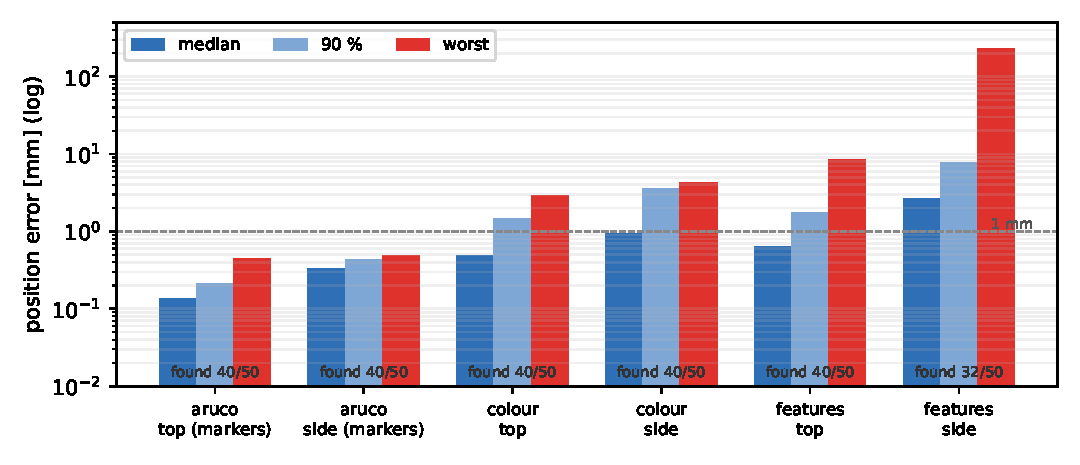
\includegraphics[width=\linewidth]{figures/errors.pdf}
\captionof{figure}{Error per method and camera pose (log scale). Only ArUco stays under 1\,mm, also in dark, noisy and
shadowed photos.}

\begin{minipage}[t]{0.49\linewidth}\centering
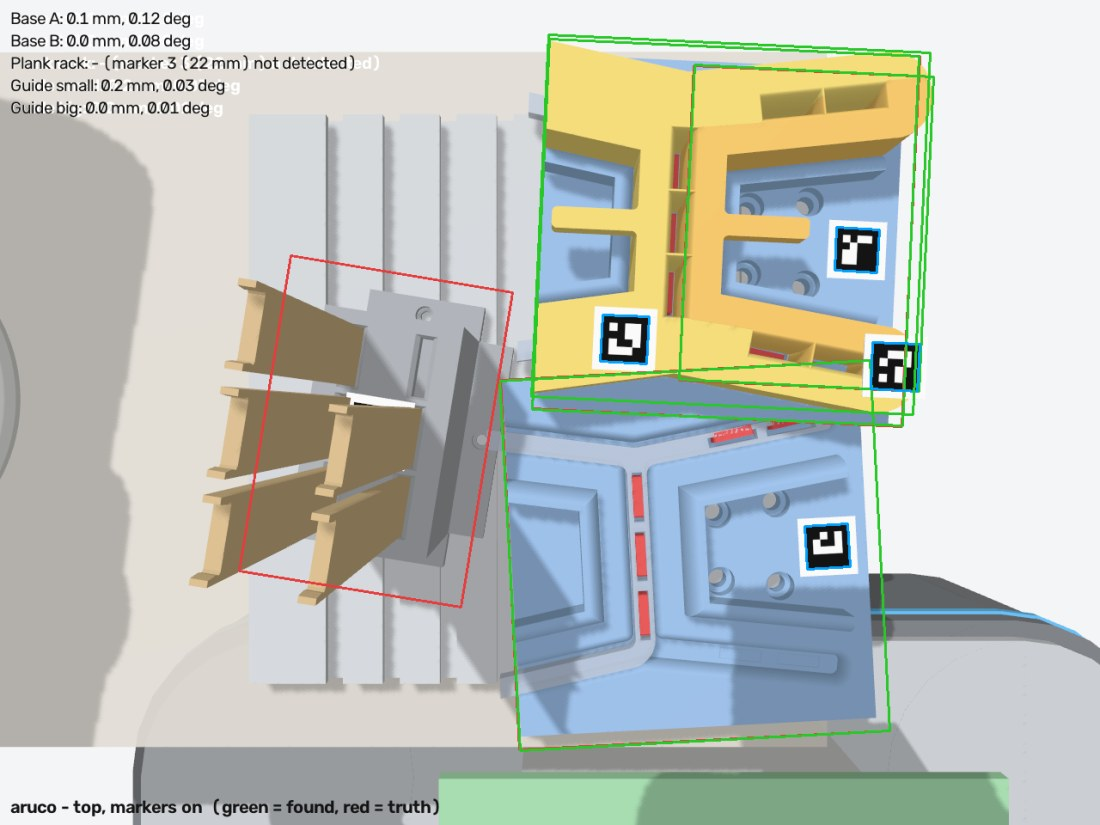
\includegraphics[width=\linewidth]{figures/aruco_top.jpg}
\captionof{figure}{ArUco: every marker found (green).}
\end{minipage}\hfill
\begin{minipage}[t]{0.49\linewidth}\centering
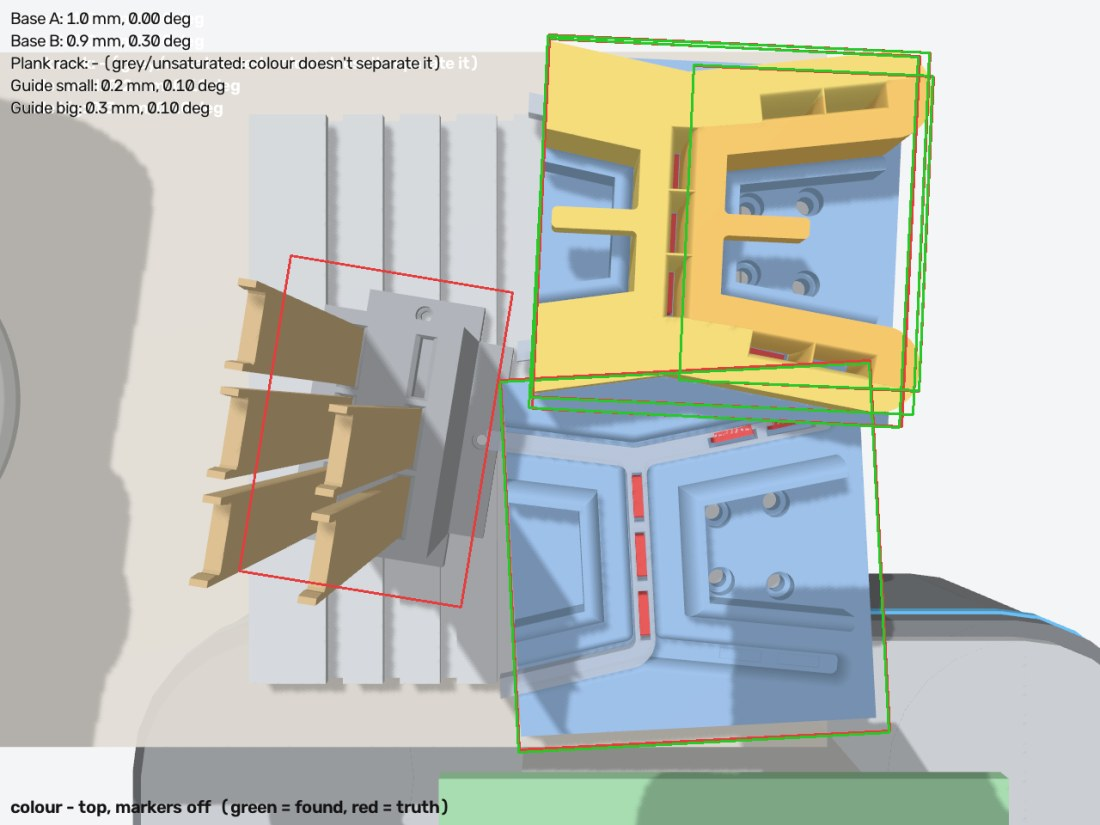
\includegraphics[width=\linewidth]{figures/colour_top.jpg}
\captionof{figure}{Colour: the two blue bases blur together.}
\end{minipage}

\newpage
\step{Calibration: step 1 -- jigs out, board flat on the empty plate}
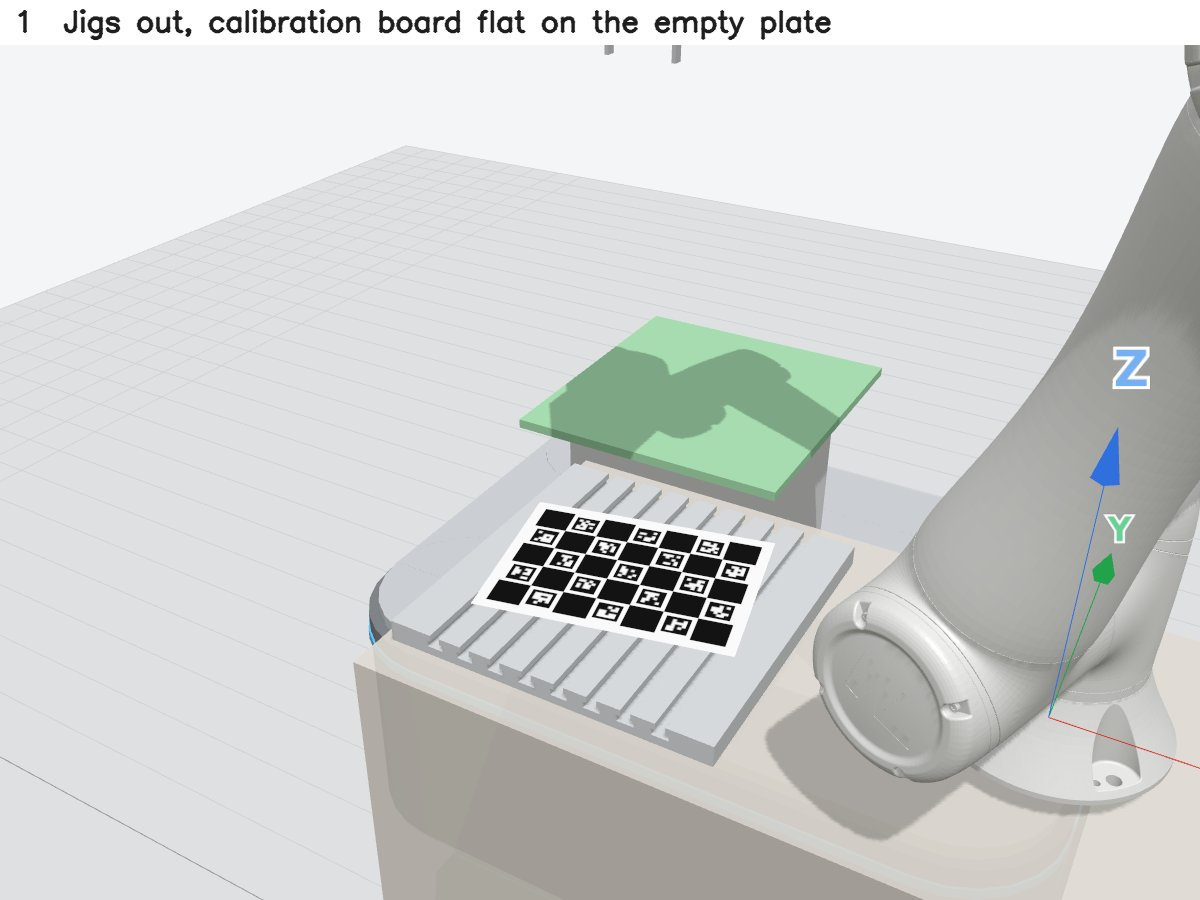
\includegraphics[width=\linewidth]{figures/wt_s1_board.jpg}
\captionof{figure}{The sim's \emph{Camera calibration} mode (orange banner, timer): jigs hidden, ChArUco board on the plate.}

\step{Step 2 -- 15 photos: board still, robot tilted 10--20\,°}
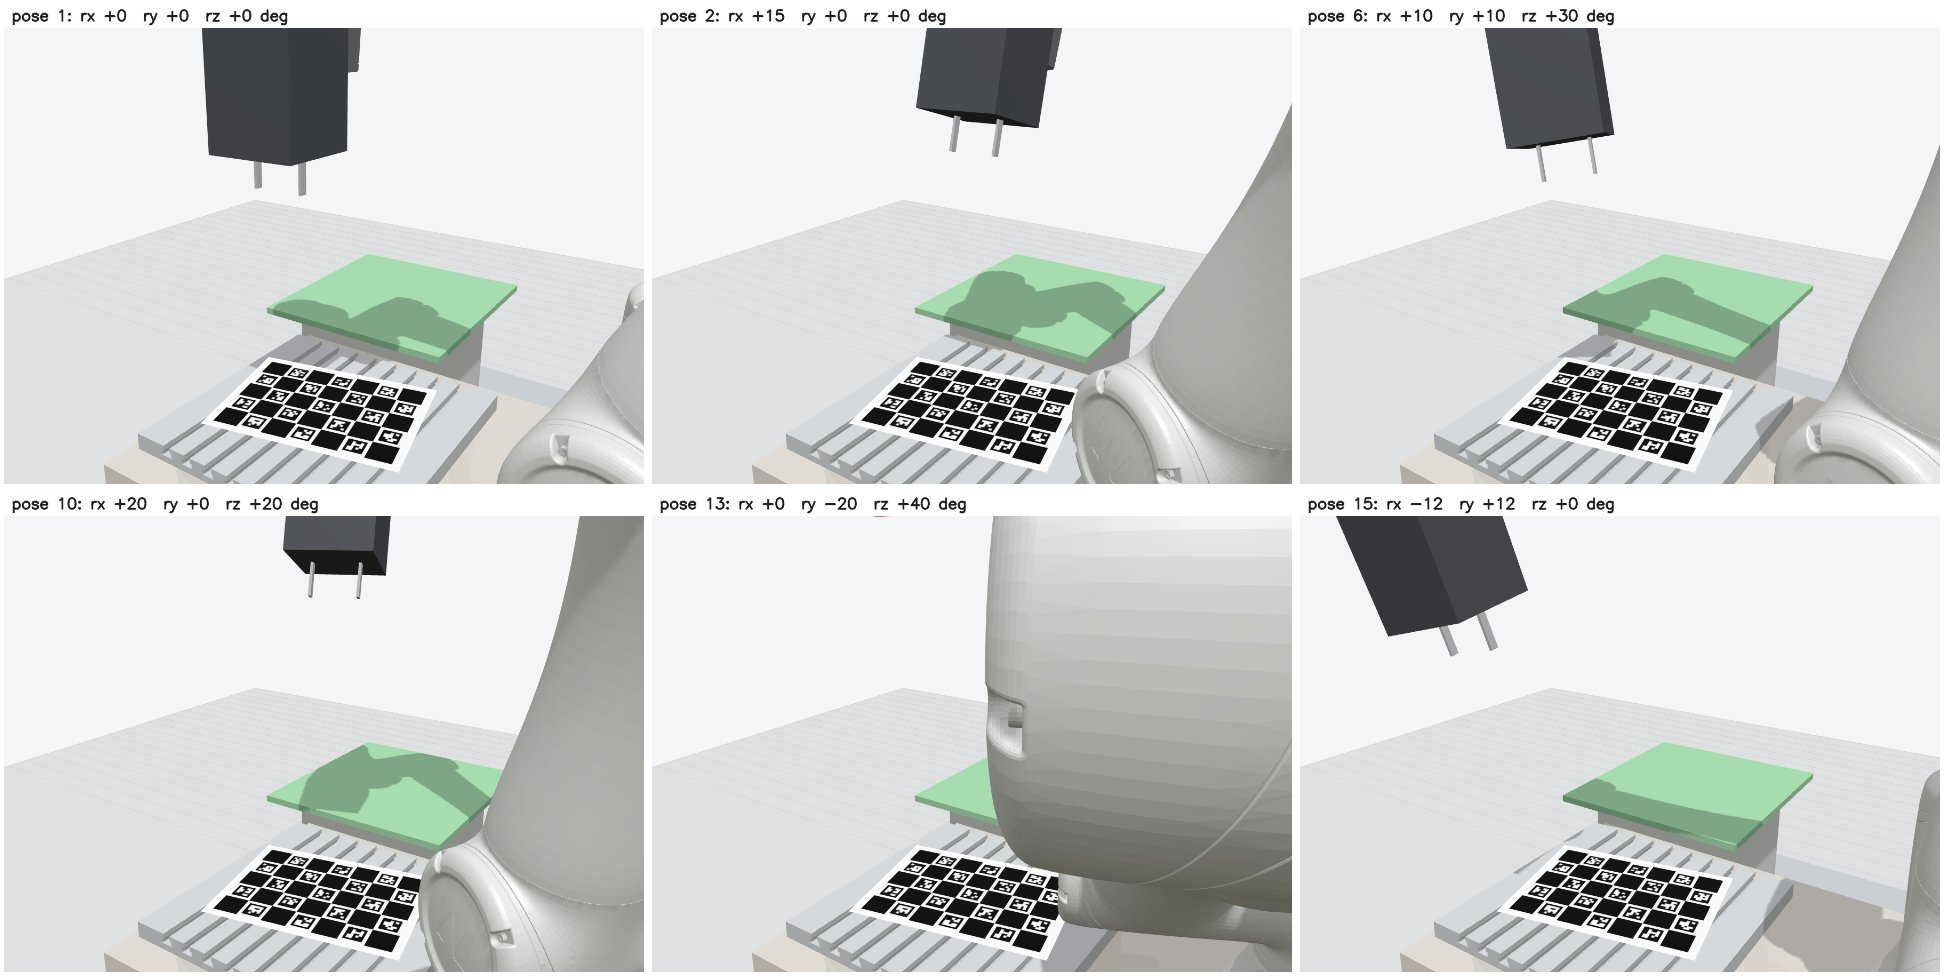
\includegraphics[width=\linewidth]{figures/wt_s2_poses_robot.jpg}
\captionof{figure}{Six of the \wtPhotos{} robot poses.}
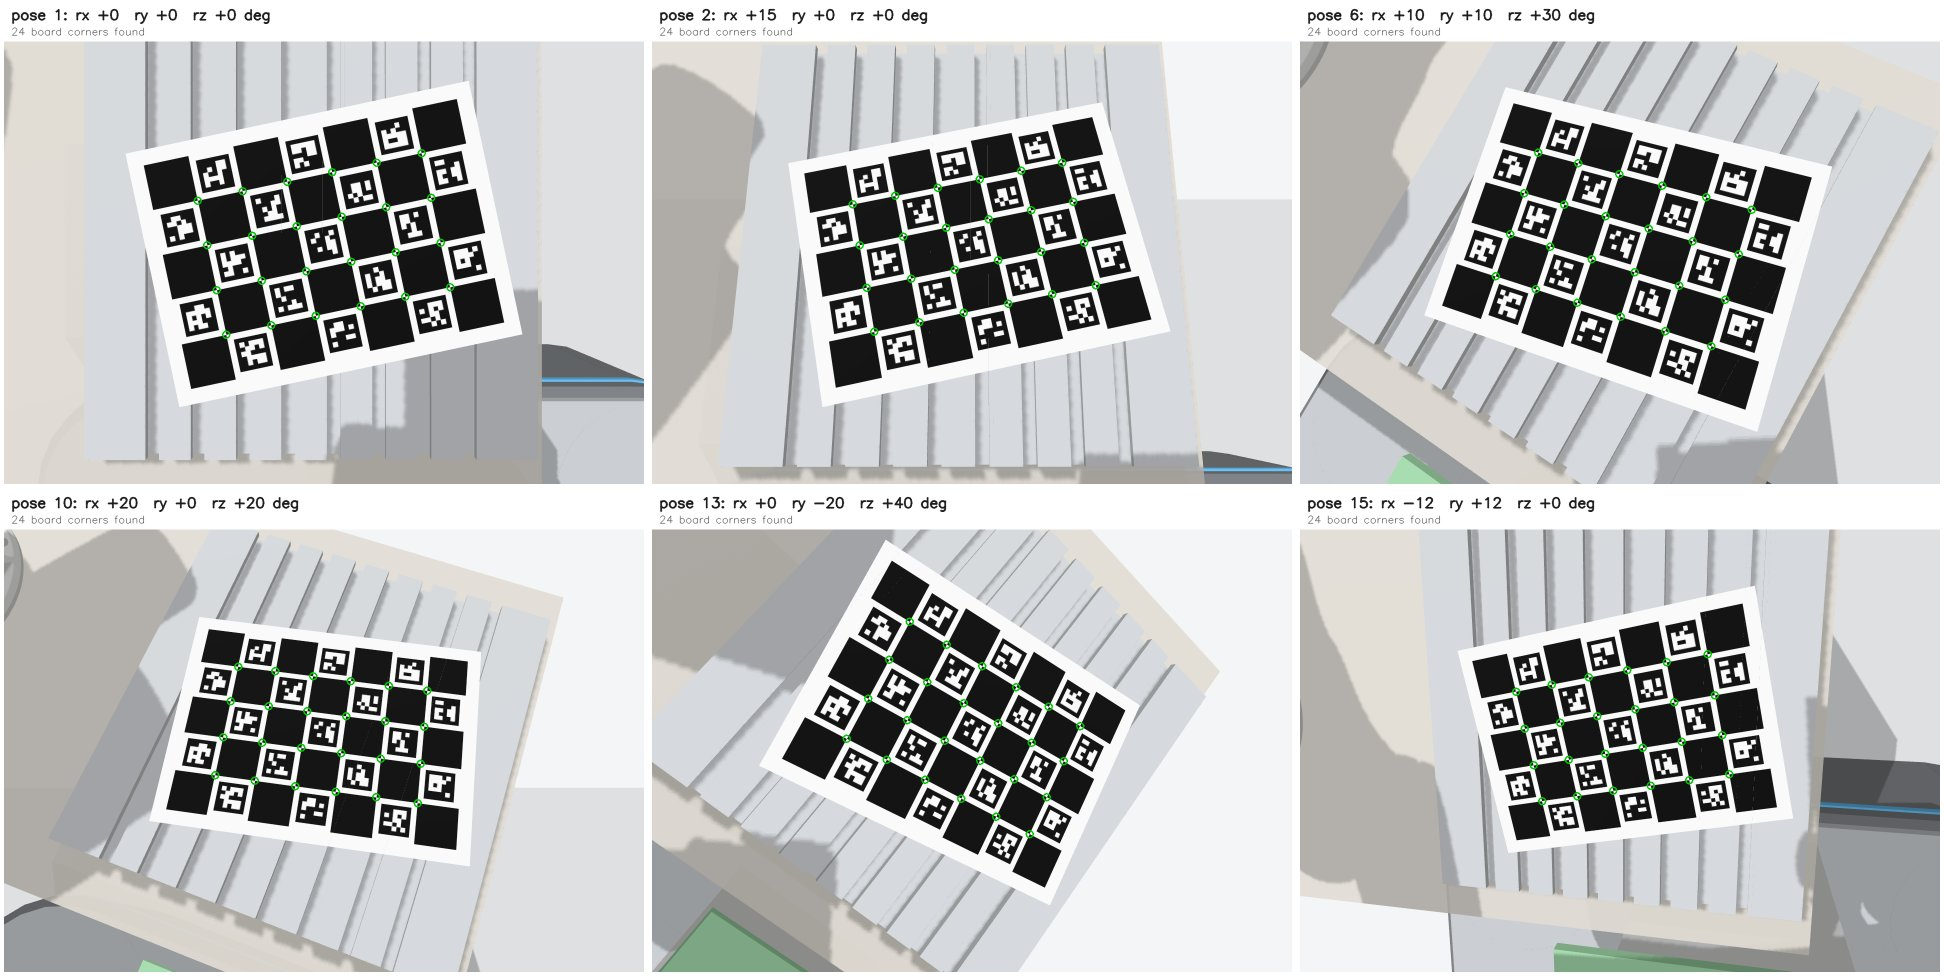
\includegraphics[width=\linewidth]{figures/wt_s2_poses_camera.jpg}
\captionof{figure}{What the tool camera saw; green = board corners found.
\textbf{Step 3:} lens + hand-eye $\rightarrow$ \code{camera.json}: reprojection \wtRms\,px, camera found at
(\wtHeFound)\,mm on the flange, \wtHePos\,mm from the truth.}

\newpage
\step{Step 4 -- jigs back in where the program was taught: two photos}
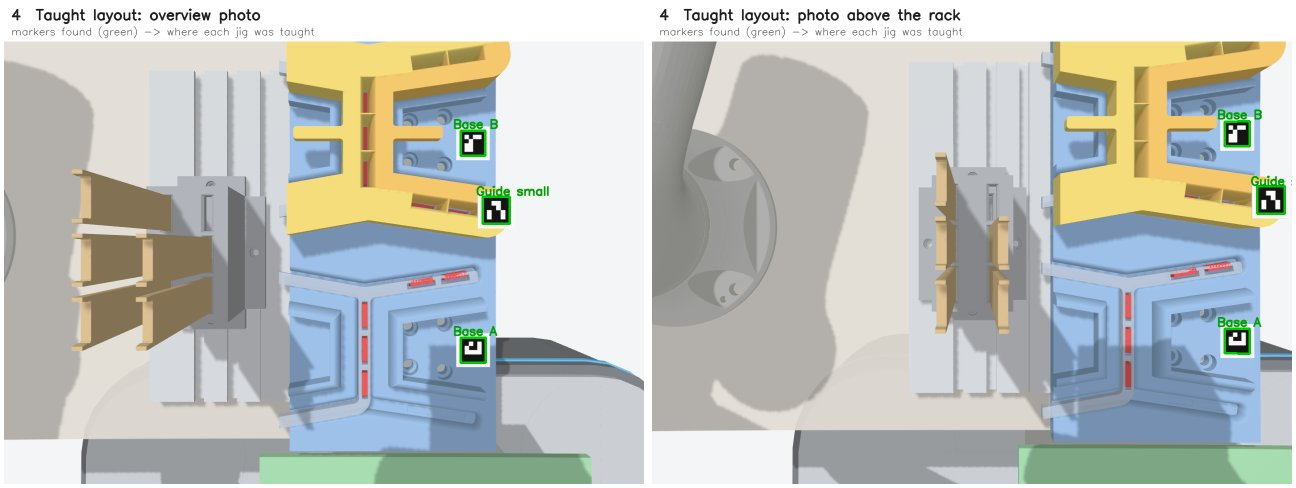
\includegraphics[width=\linewidth]{figures/wt_s4_taught.jpg}
\captionof{figure}{Overview + straight above the rack (the planks hide its marker from the side). Every marker found
$\rightarrow$ \code{real\_jigs.json}.}

\step{Step 5 -- the bases are put down somewhere else (moved and turned; the rack stays)}
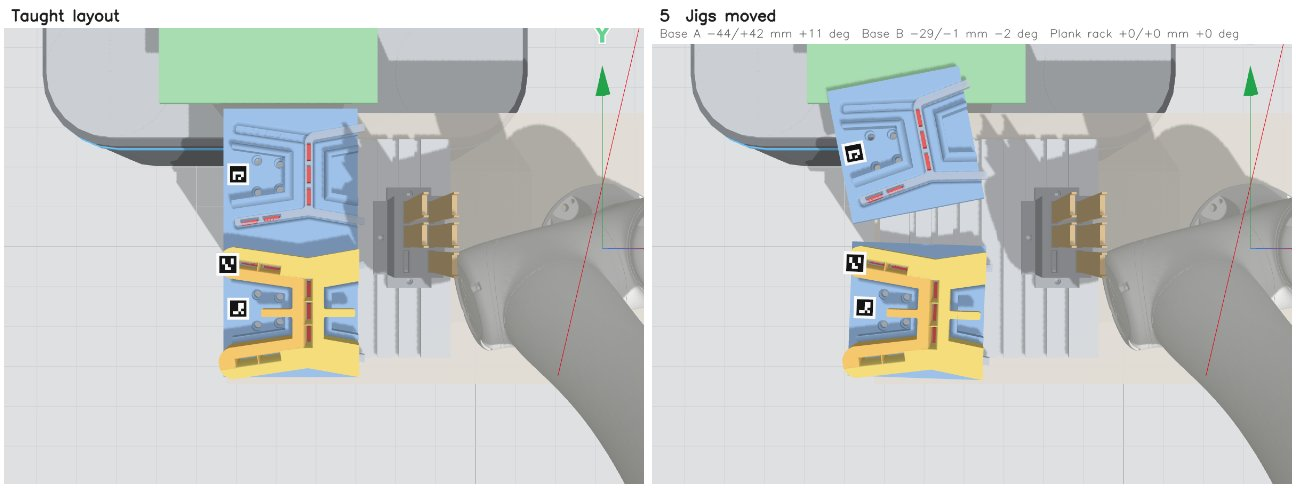
\includegraphics[width=\linewidth]{figures/wt_s5_moved.jpg}
\captionof{figure}{Before / after, seen from above.}

\step{Step 6 -- measure: the same two photos again}
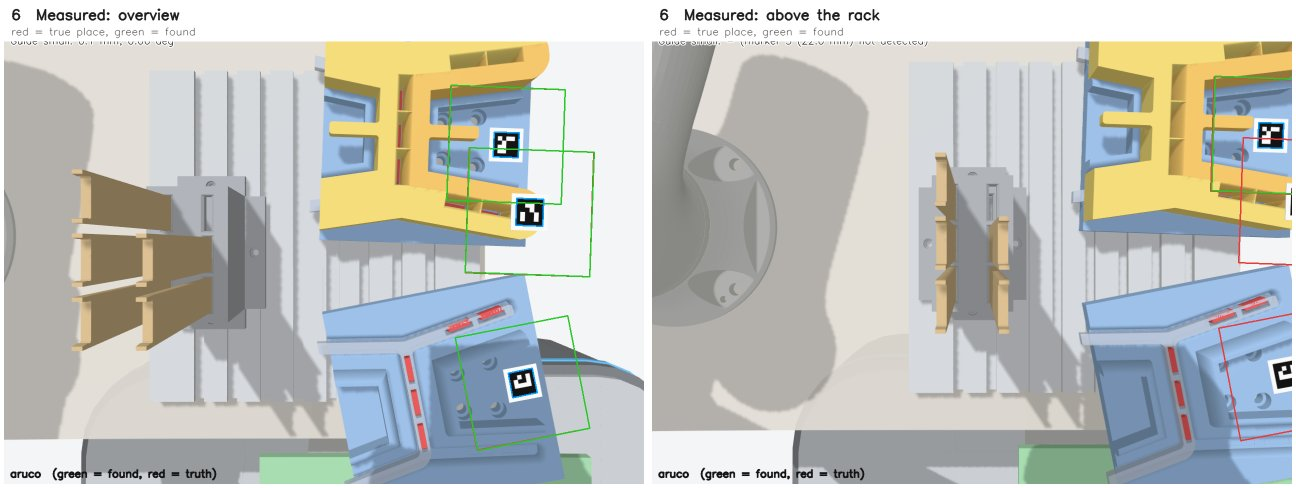
\includegraphics[width=\linewidth]{figures/wt_s6_measured.jpg}
\captionof{figure}{Red = true place, green = found (they overlap). Set: Base A \wtSetA, Base B \wtSetB{} (about each
jig's centre); the rack has no marker and stays. Found within \textbf{\wtMeasMax\,mm} at the markers.}

\newpage
\step{Steps 7--8 -- V10: every taught point moved with its jig}
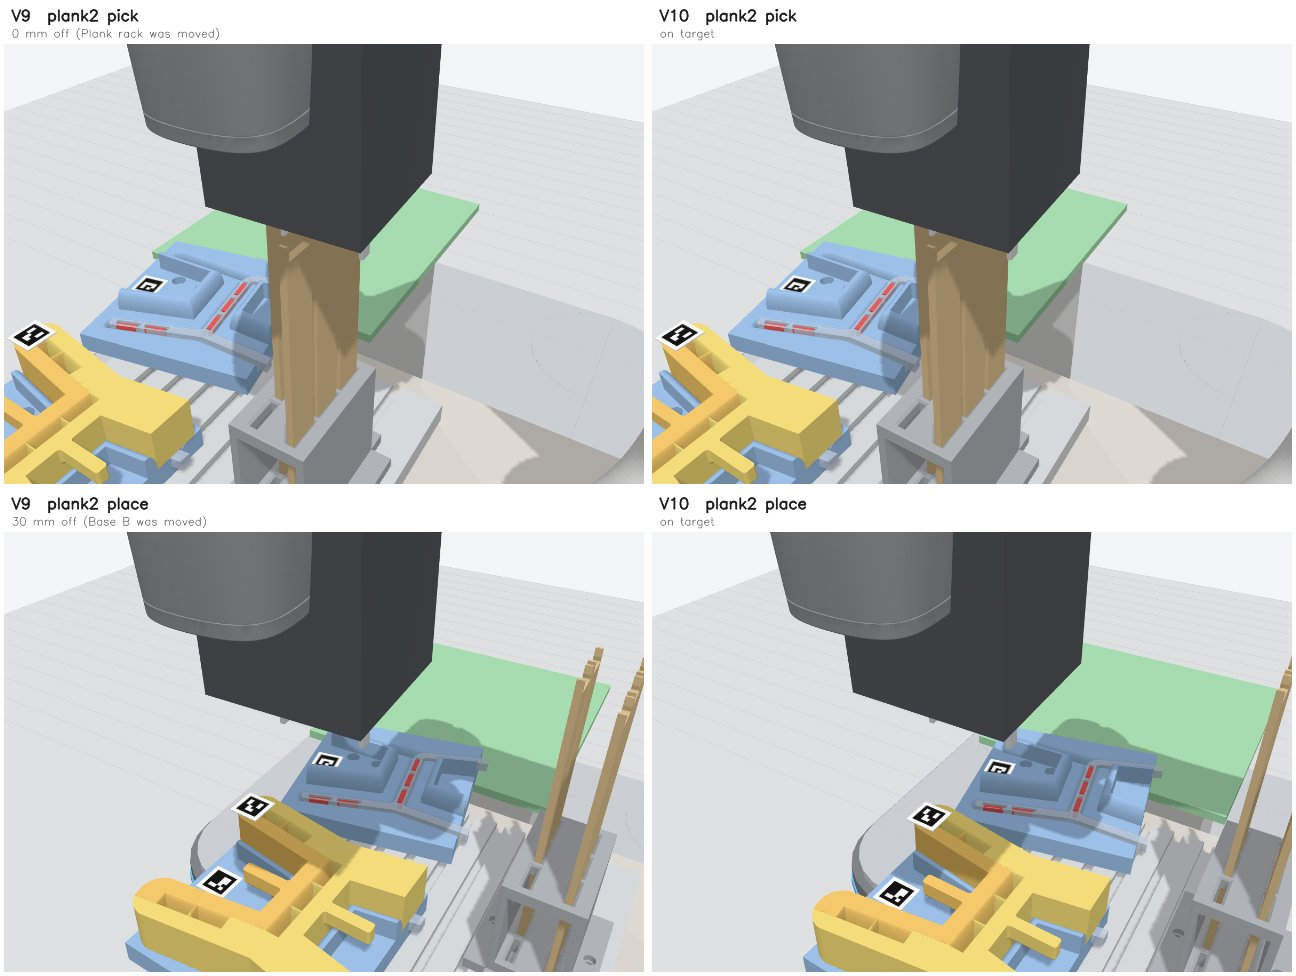
\includegraphics[width=\linewidth]{figures/wt_s8_v9_vs_v10.jpg}
\captionof{figure}{The same grip and place on the moved jigs. V9 (taught points) misses; V10 is on target. Over all
\wtMoves{} moves above a jig: V10 within \wtTipMax\,mm (median \wtTipMed), V9 up to \wtVnineMax\,mm off.
Collision check with the jigs where they are now -- V9: \wtCollNine; V10: \wtCollTen.}

\newpage
\step{Step 9 -- V10 assembles the bench on the moved jigs (\wtAsmEvents{} grabs and releases, run: \wtAsmState)}
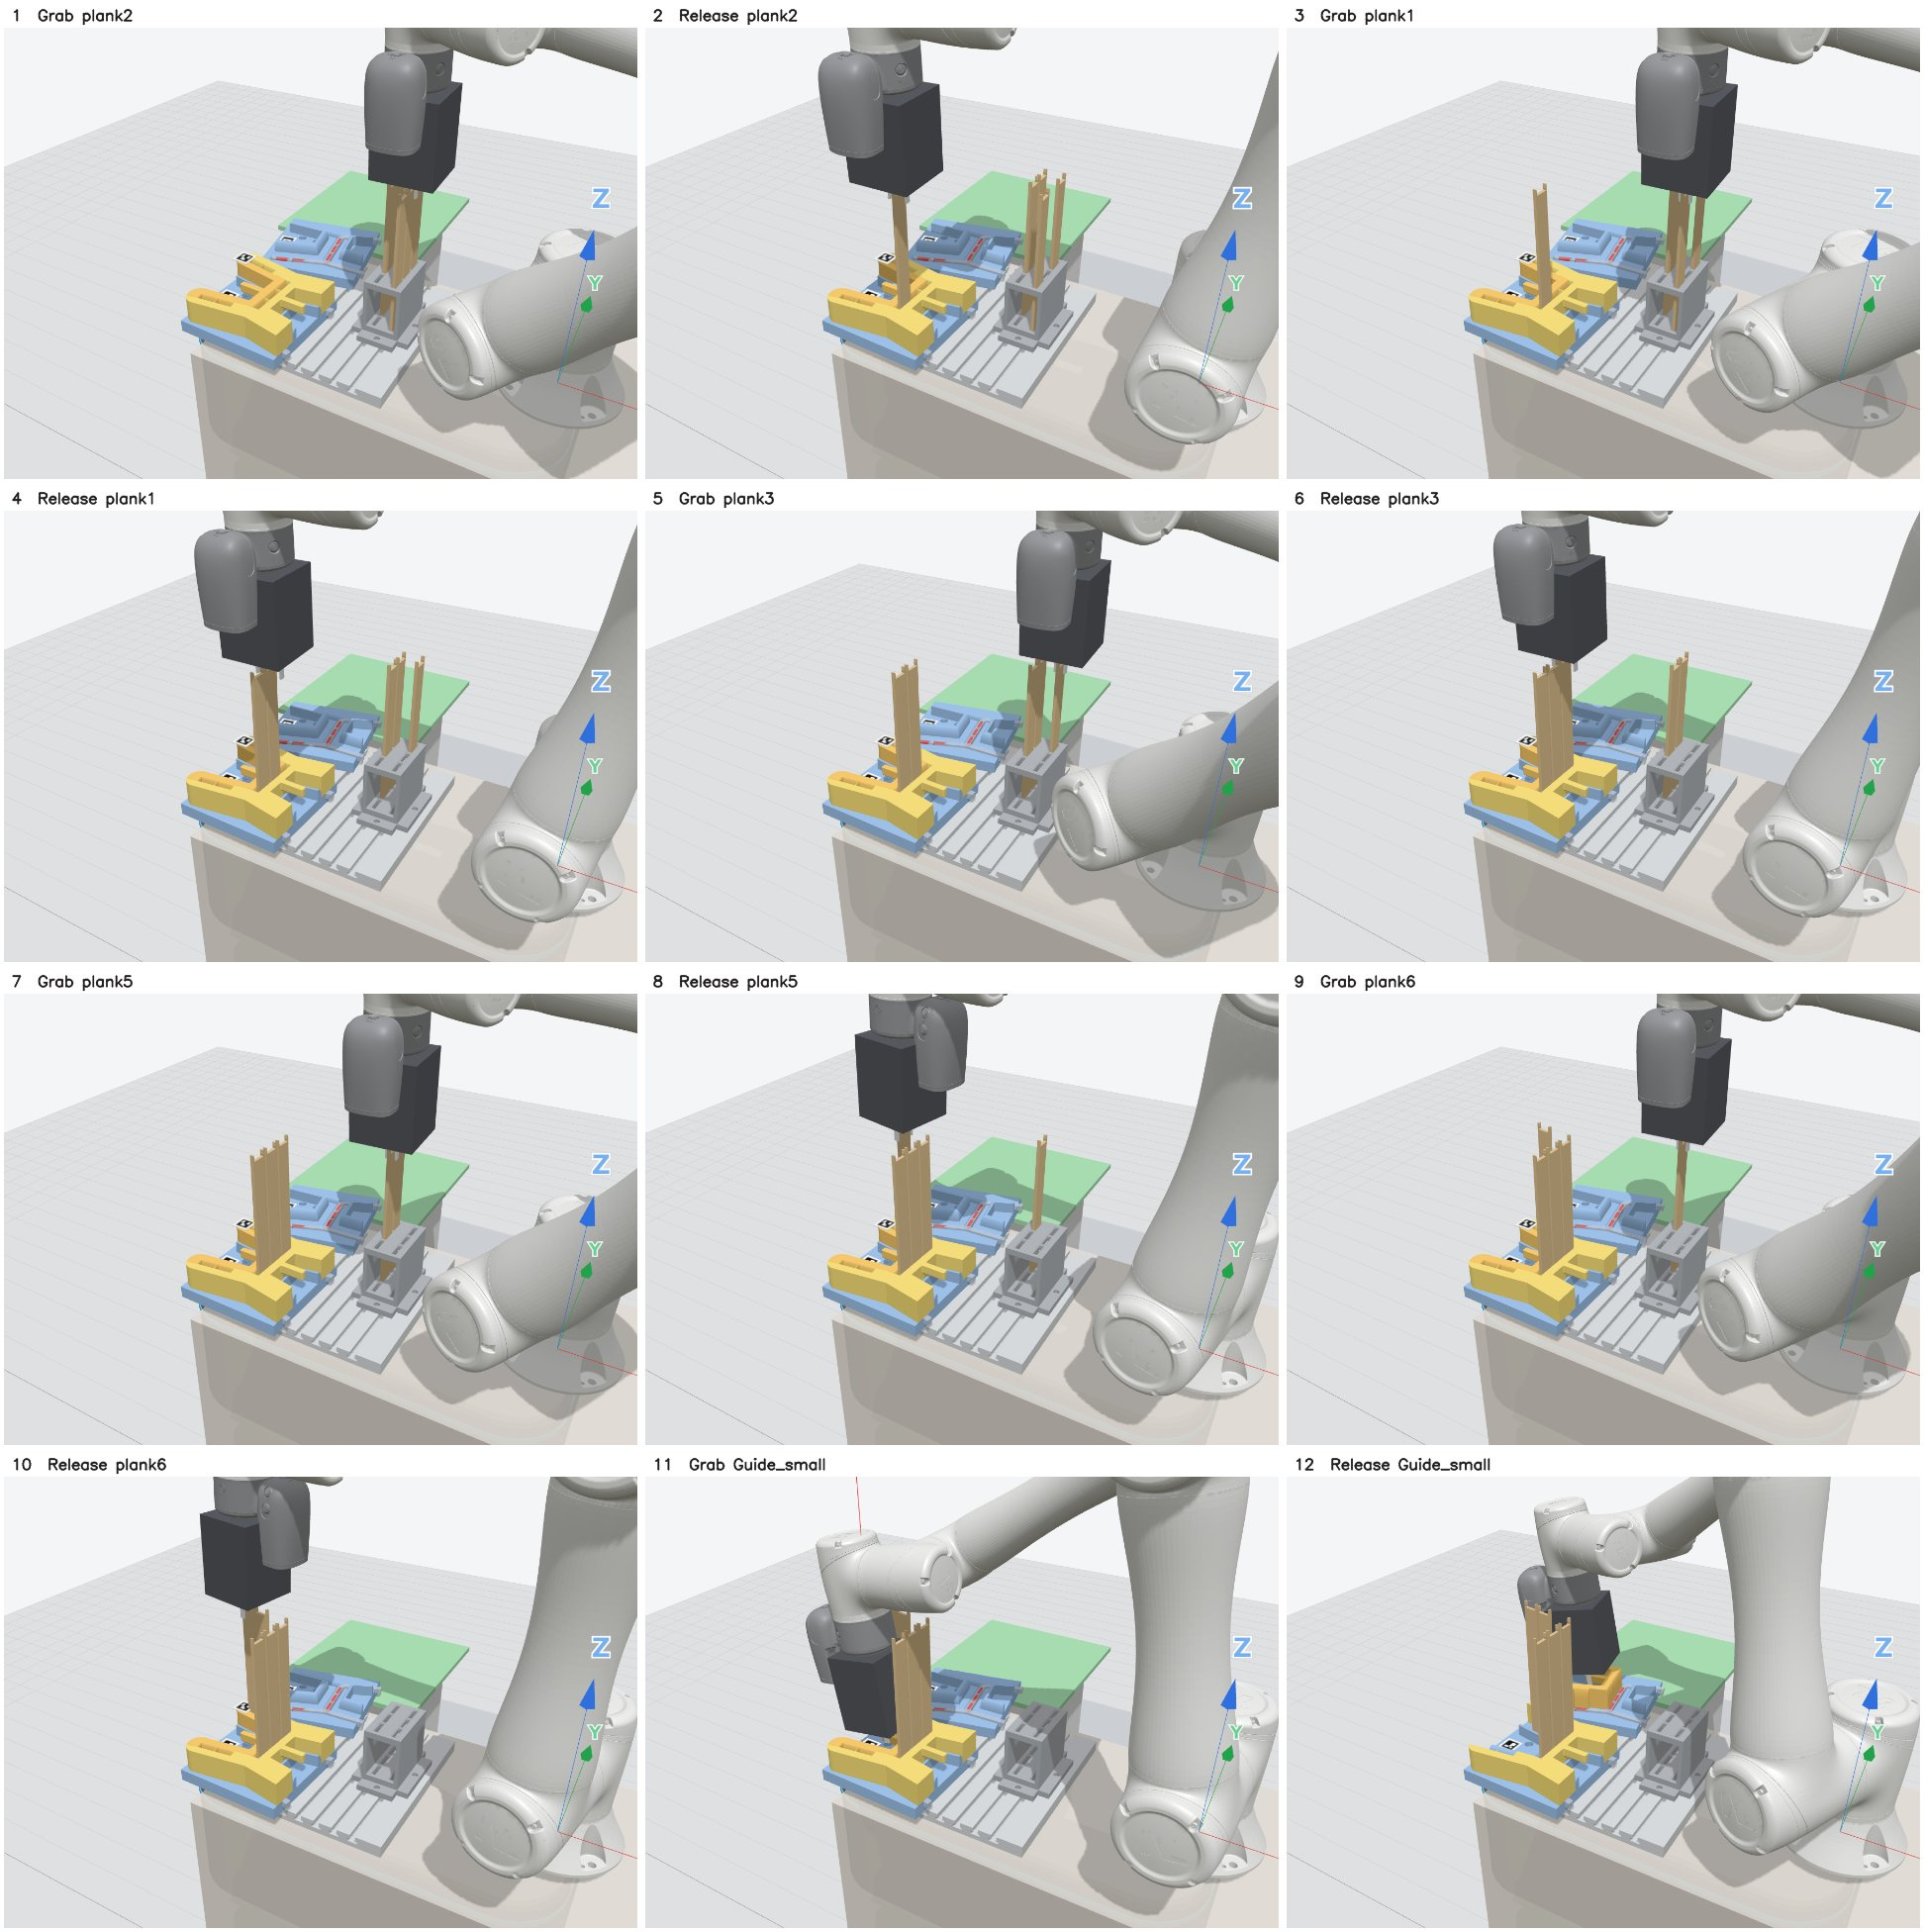
\includegraphics[width=\linewidth]{figures/wt_s9_assembly_1.jpg}
\captionof{figure}{V10 assembly, sheet 1 of 2: a picture at every grab and release.}
\newpage
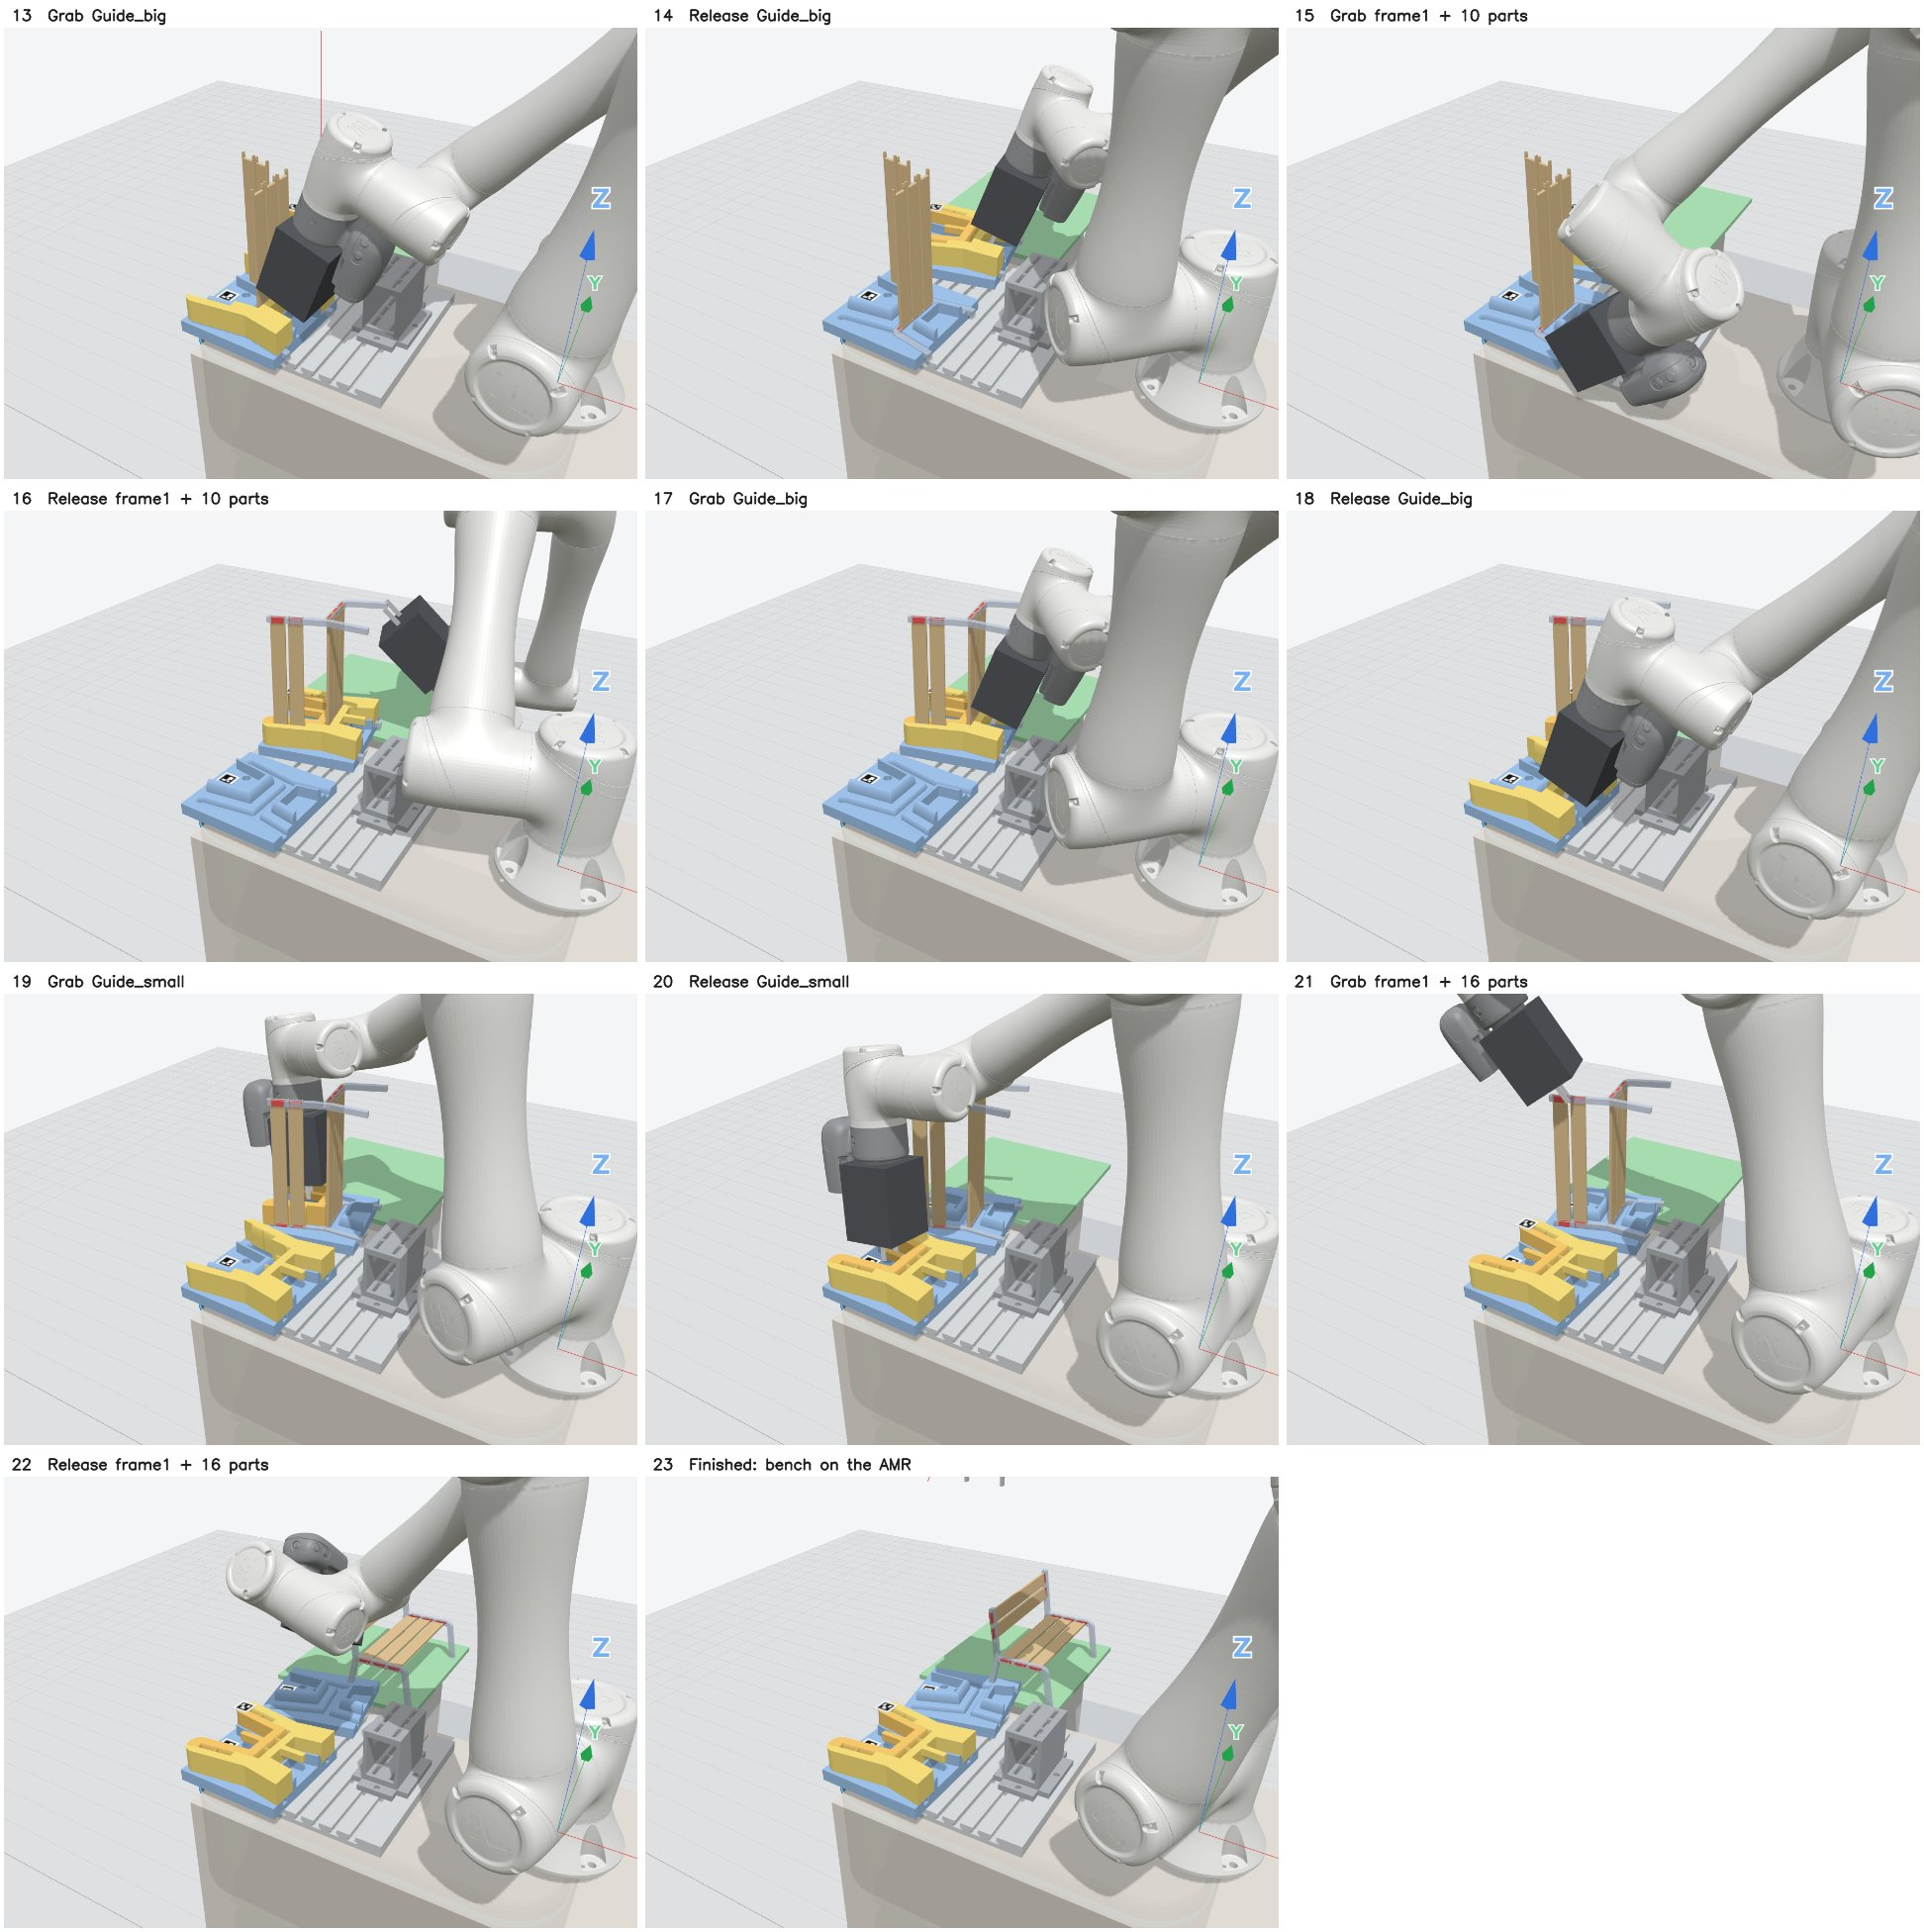
\includegraphics[width=\linewidth]{figures/wt_s9_assembly_2.jpg}
\captionof{figure}{V10 assembly, sheet 2 of 2: a picture at every grab and release.}


\newpage
\step{In the lab -- checklist}
\begin{enumerate}[leftmargin=6mm,itemsep=2pt]
\item Print \code{print\_markers.py}: 3 jig markers (Base A, Base B, guide) + ChArUco board, 100\,\% scale, matte
paper. Check the 100\,mm bar. The plank rack stays bolted where it was taught.
\item TM camera: TMflow vision job $\rightarrow$ \emph{External Detection} $\rightarrow$ \code{http://<laptop>:6189};
run \code{tm\_camera.py calib}; see \code{tm\_camera.log}. (No such step? Use a USB webcam + \code{real\_capture.py}.)
\item \textbf{Jigs off.} Board glued on a stiff plate, flat on the empty T-slot plate.
\item 15 photos, board still, robot tilted 10--20\,° (jog by hand, slow, from above) $\rightarrow$
\code{calibrate.py intrinsics}, then \code{calibrate.py handeye}.
\item \textbf{Jigs back} where the program was taught. Markers glued flat; measure each marker's height with the TCP.
\item Overview photo + photo above the rack $\rightarrow$ \code{real\_setup.py \dots{} -{}-z "Base A=\dots"}.
\item Check: move one jig 10\,mm along a T-slot, 2 photos, \code{jig\_vision.py \dots{} -{}-save moves.json}: must
read $\approx$10\,mm.
\item \code{python bench\_cell\_v10.py moves.json} $\rightarrow$ V10. Run it in the sim first (preset V10), then on the
robot at low speed.
\end{enumerate}

\medskip
\textbf{Limits.} The sim camera is ideal: expect real errors a few times larger (still well under the grip tolerance if
near 1\,mm). Only plane moves (x, y, rz) are measured; the rack (no marker) must not move.
Each new layout gets a collision check (\code{collision\_for\_run.py}) before the robot runs it. The frame flip in stage 4 is the one big rotation in the program:
its wrist is near a singularity, so check V10's flip in the sim before the robot.
All numbers: \code{jig\_vision\_report\_detailed.pdf}; run: \code{\wtRun}.
\end{document}
